\documentclass{article}
\usepackage{graphicx}
\usepackage[margin=1.5cm]{geometry}
\usepackage{amsmath}

\begin{document}
\twocolumn

\title{Monday Warm Up: Unit 4, Mutual Inductance, Self-inductance, and RL circuits}
\author{Prof. Jordan C. Hanson}

\maketitle

\section{Memory Bank}

\begin{itemize}
\item $\epsilon = -L \Delta I /\Delta t$ ... Faraday's Law
\item $\epsilon(t) = \epsilon_0 \sin(\omega t)$ ... AC voltage generated by generator.  $\epsilon_0$ is proportional to $\omega$.
\item $P_{max} = V_{max}^2/R$ ... Max power of an AC generator.
\item $P_{ave} = \frac{1}{2} P_{max}$ ... Average power of an AC generator.
\item $T = 1/f$ ... Inverse relationship between frequency and period.
\item 1 H = 1 $\Omega$ s ... The \textit{Henry} is a unit of inductance, often represented by $L$.
\item $I(t) = I_0\left(1 - \exp(-t/\tau)\right)$ ... Current when RL circuits turn on ($\tau = R/L$).
\item $I(t) = I_0\exp(-t/\tau)$ ... Current when RL circuits turn off ($\tau = R/L$).
\end{itemize}

\section{Mutual Inductance}

\begin{enumerate}
\item Consider Fig. \ref{fig:coils}.  If the coils of the heating element for an electric dryer are \textit{counter-wound}, why does this reduce back emf when the current is increased? \\ \vspace{1cm}
\end{enumerate}

\section{Self-Inductance}

\begin{enumerate}
\item Consider Fig. \ref{fig:coils2}.  (a) What is the back emf in across an inductor with $L=50$ mH, if the current is increased from 0 to 2 A in 0.2 seconds? (b) What is the emf across the inductor if the current is shut off in 0.2 seconds? (d) How do you think it works if two inductors are in series? \\ \vspace{3cm}
\item What is the inductance of a device, if we measure a 20 mV back emf for an increasing current of 100 mA per second? \\ \vspace{2cm}
\end{enumerate}

\begin{figure}
\centering
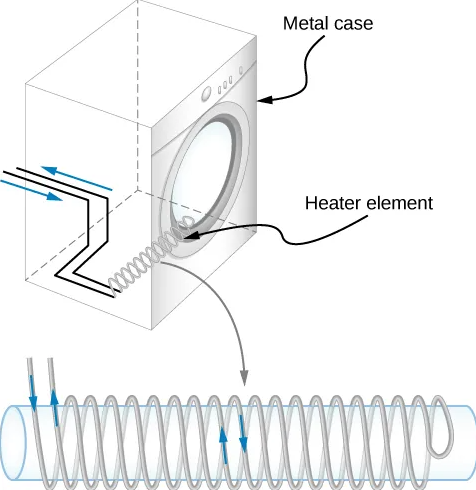
\includegraphics[width=0.3\textwidth]{figures/coils.png}
\caption{\label{fig:coils} Coils wrapped around the outside of a solenoid.}
\end{figure}

\begin{figure}
\centering
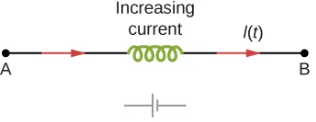
\includegraphics[width=0.3\textwidth]{figures/coils2.png}
\caption{\label{fig:coils2} Back emf of an inductor with increasing current.}
\end{figure}

\section{RL Circuits}

\begin{enumerate}
\item (a) What is the characteristic time constant for a 9.0 mH inductor in series with a 3.00 $\Omega$ resistor? (b) Find the current 6.00 ms after the circuit is closed. (c) What will be the current if the circuit is left closed indefinately?
\end{enumerate}

\end{document}
